\documentclass[border=10pt,tikz]{standalone}
\usepackage{tikz}
\usepackage{xcolor}
\usepackage[T1]{fontenc}
\usepackage{lmodern}
\usetikzlibrary{positioning,arrows.meta,decorations.pathreplacing,shapes.geometric,calc,fadings,fit,backgrounds,shadows}

\definecolor{ink}{HTML}{0E1116}
\definecolor{inksoft}{HTML}{3A3F47}
\definecolor{inkmute}{HTML}{6A7079}
\definecolor{textc}{HTML}{2563EB}
\definecolor{audioc}{HTML}{EA580C}
\definecolor{accentc}{HTML}{7C3AED}
\definecolor{audiogreen}{HTML}{059669}
\definecolor{linec}{HTML}{CFC9B8}
\definecolor{soft}{HTML}{F3F1EA}

\begin{document}
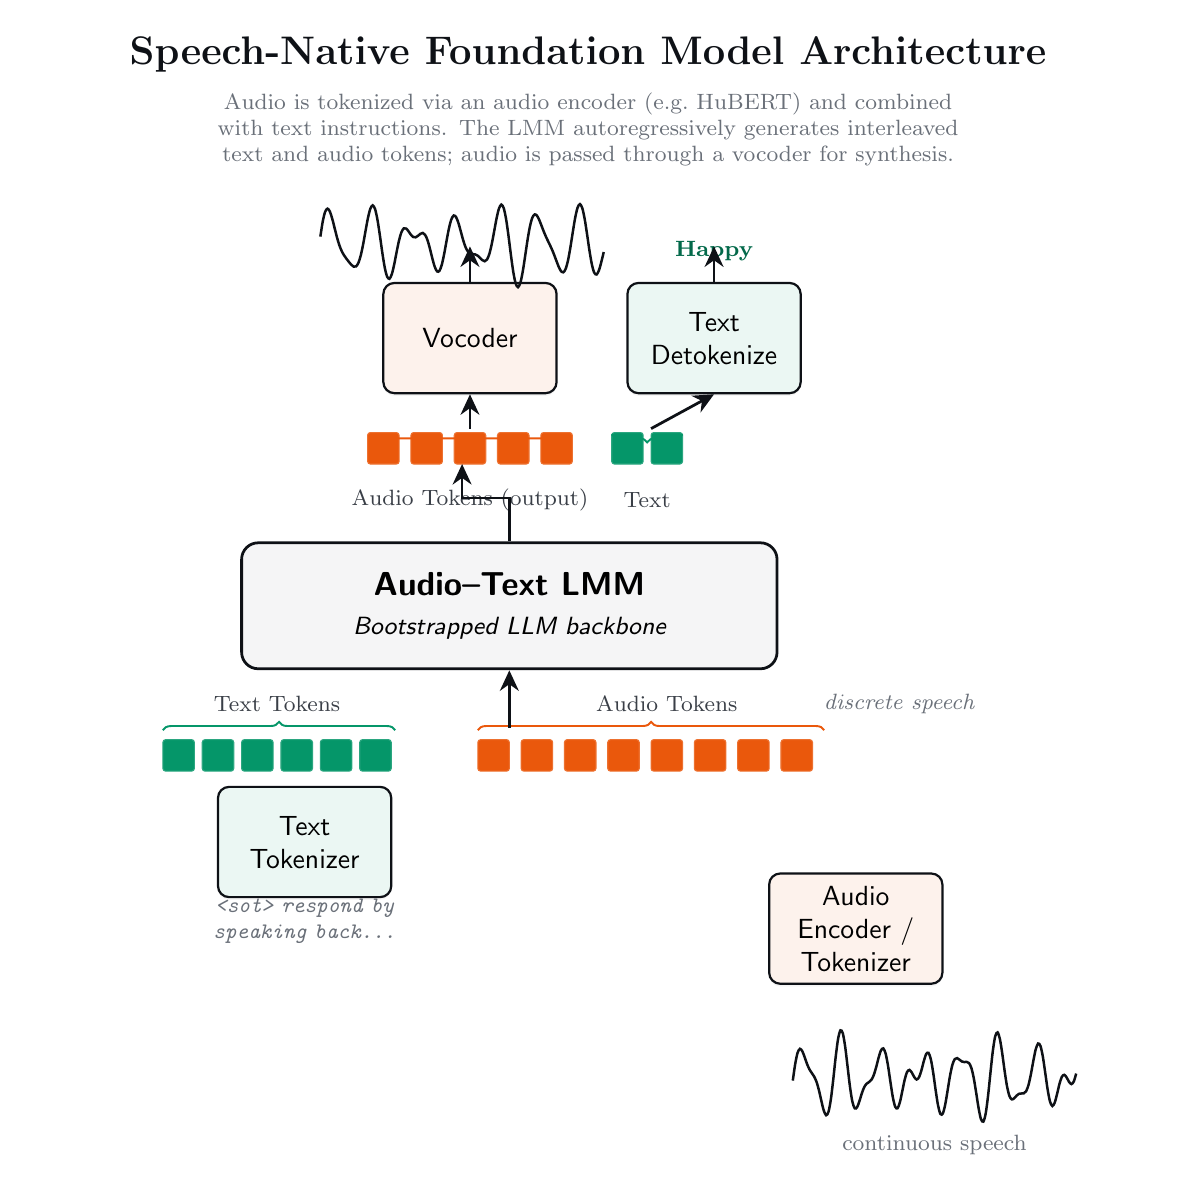
\begin{tikzpicture}[
  font=\sffamily,
  every node/.style={font=\sffamily},
  module/.style={
    rectangle, rounded corners=4pt,
    draw=ink, line width=0.8pt,
    fill=white, drop shadow={shadow xshift=0pt, shadow yshift=-1pt, opacity=0.08},
    minimum height=14mm, minimum width=22mm, align=center,
    inner sep=4pt
  },
  bigmod/.style={
    rectangle, rounded corners=6pt,
    draw=ink, line width=1pt,
    fill=ink!4, minimum height=16mm, minimum width=68mm, align=center
  },
  audiotok/.style={
    rectangle, rounded corners=1pt, draw=audioc!85, fill=audioc, minimum width=4mm, minimum height=4mm, inner sep=0pt
  },
  texttok/.style={
    rectangle, rounded corners=1pt, draw=audiogreen!85, fill=audiogreen, minimum width=4mm, minimum height=4mm, inner sep=0pt
  },
  arr/.style={->, >={Stealth[length=2.6mm,width=2.4mm]}, line width=1pt, draw=ink},
  thinarr/.style={->, >={Stealth[length=1.8mm,width=1.6mm]}, line width=0.6pt, draw=inkmute}
]

% --- INPUT SIDE (bottom) ---
% Audio waveform (input)
\begin{scope}[shift={(2.6,-3.4)}]
  \draw[draw=ink, line width=0.9pt] plot[domain=0:3.6, samples=120, smooth]
    (\x, {0.32*sin(720*\x) + 0.18*sin(1280*\x + 30) - 0.12*sin(900*\x + 90)});
  \node[font=\footnotesize, color=inkmute] at (1.8,-0.85) {continuous speech};
\end{scope}

% Text Tokenizer
\node[module, fill=audiogreen!8] (texttok) at (-3.6,-0.4) {Text\\Tokenizer};
\node[font=\footnotesize\itshape, color=inkmute, text width=3.4cm, align=center, anchor=north] at (-3.6,-1.0) {\texttt{<sot> respond by speaking back\dots}};

% Audio Encoder/Tokenizer
\node[module, fill=audioc!8] (audtok) at (3.4,-1.5) {Audio\\Encoder /\\Tokenizer};

% Token sequences after tokenization
% Text tokens (green)
\foreach \i in {0,1,2,3,4,5} {
  \node[texttok] at (-5.2 + 0.5*\i, 0.7) {};
}
\node[font=\footnotesize, color=inksoft] at (-3.95,1.35) {Text Tokens};

% Audio tokens (orange)
\foreach \i in {0,1,2,3,4,5,6,7} {
  \node[audiotok] at (-1.2 + 0.55*\i, 0.7) {};
}
\node[font=\footnotesize, color=inksoft] at (1.0,1.35) {Audio Tokens};
\node[font=\footnotesize\itshape, color=inkmute] at (3.95,1.35) {discrete speech};

% Joint sequence brackets
\draw[decorate, decoration={brace, amplitude=3pt, raise=2pt}, draw=audiogreen, line width=0.7pt] (-5.4,0.95) -- (-2.45,0.95);
\draw[decorate, decoration={brace, amplitude=3pt, raise=2pt}, draw=audioc, line width=0.7pt] (-1.4,0.95) -- (3.0,0.95);

% --- LMM ---
\node[bigmod] (lmm) at (-1.0, 2.6) {\large \textbf{Audio--Text LMM}\\[2pt] {\small\itshape Bootstrapped LLM backbone}};

% Arrow into LMM from joint tokens
\draw[arr] (-1.0,1.05) -- (-1.0, 1.78);

% --- OUTPUT SIDE ---
% Output tokens (interleaved)
\foreach \i in {0,1,2,3,4} {
  \node[audiotok] at (-2.6 + 0.55*\i, 4.6) {};
}
\foreach \i in {0,1} {
  \node[texttok] at (0.5 + 0.5*\i, 4.6) {};
}
\node[font=\footnotesize, color=inksoft] at (-1.5,3.95) {Audio Tokens (output)};
\node[font=\footnotesize, color=inksoft] at (0.75,3.95) {Text};

\draw[decorate, decoration={brace, amplitude=3pt, raise=2pt, mirror}, draw=audioc, line width=0.7pt] (-2.7,4.85) -- (-0.4,4.85);
\draw[decorate, decoration={brace, amplitude=3pt, raise=2pt, mirror}, draw=audiogreen, line width=0.7pt] (0.3,4.85) -- (1.2,4.85);

\draw[arr] (lmm.north) -- ++(0,0.55) -| (-1.6,4.4);

% Vocoder
\node[module, fill=audioc!8] (voc) at (-1.5,6.0) {Vocoder};
\draw[arr] (-1.5,4.85) -- (voc.south);

% Output waveform
\begin{scope}[shift={(-3.4,7.2)}]
  \draw[draw=ink, line width=0.9pt] plot[domain=0:3.6, samples=120, smooth]
    (\x, {0.32*sin(680*\x) + 0.16*sin(1100*\x + 50) - 0.10*sin(820*\x + 160)});
\end{scope}
\draw[arr] (voc.north) -- ++(0,0.45);

% Text Detokenize
\node[module, fill=audiogreen!8] (detok) at (1.6,6.0) {Text\\Detokenize};
\draw[arr] (0.8,4.85) -- (detok.south);
\node[font=\footnotesize\bfseries, color=audiogreen!70!black] at (1.6,7.1) {Happy};
\draw[arr] (detok.north) -- ++(0,0.45);

% Title
\node[font=\Large\bfseries, color=ink] at (0,9.6) {Speech-Native Foundation Model Architecture};
\node[font=\footnotesize, color=inkmute, text width=14cm, align=center] at (0,8.65) {Audio is tokenized via an audio encoder (e.g.\ HuBERT) and combined with text instructions. The LMM autoregressively generates interleaved text and audio tokens; audio is passed through a vocoder for synthesis.};

\end{tikzpicture}
\end{document}
